\section{Projektplanung / -Management}

Das Projektteam 32 besteht aus sieben Personen, die sich auf folgende 
Studienrichtungen aufteilen: Drei Personen Maschinentechnik, drei 
Personen Informatik und eine Person Elektrotechnik. Die Studienrichtungen 
sind sogleich die jeweiligen Verantwortungen. In den Bereichen mit mehreren 
Projektmitgliedern wird die Verantwortung für Teilaufgaben jeweils 
situativ verteilt. Für allgemeine Projektarbeiten ist jeweils die 
hauptverantwortliche Person bestimmt. Diese kann Teilaufgaben definieren 
und sie an andere Teammitglieder zur Bearbeitung delegieren. Die Hierarchie 
im Team ist bewusst flach und ohne eigentlichen Projektleiter gehalten. 
Entscheide werden im Plenum diskutiert und gefällt. Die Leitung oder Führung 
einer Besprechung obliegt der oder den Verantwortlichen des jeweiligen Themas. 
Mit dieser Teamstruktur ist gewährleistet, dass alle Mitglieder Verantwortung 
tragen können und müssen. Dies soll Motivation und Eigeninitiative fördern. 
Im Verlauf von PREN1 hat sich gezeigt, dass diese Projektorganisation optimal 
ist. Jedes Teammitglied hatte das gleiche Mitspracherecht, was die Kreativität 
und das Engagement wesentlich förderte. Da kein eigentlicher Projektleiter 
vorhanden war, musste jedes Teammitglied über seinen Themenbereich hinaus 
mitdenken. Es entstand eine lebhafte Diskussionskultur, die viele gute Ansätze 
und Lösungen hervorbrachte. Da dies alles eher offen und frei vonstattenging, 
waren die Aufteilung und das Vorgehen danach nicht immer allen zu 100\% klar. 
Aus diesem Grund wurden in PREN2 die sogenannten Planungssitzungen eingeführt. 
Mit diesem Instrument wurden die Besprechungen und die Beschlussfassungen, die 
sich während PREN1 ergeben haben, organisierter und vor allem strukturierter durchgeführt.
Die Planungssitzungen wurden jeweils alle zwei bis drei Wochen abgehalten. An diesen 
Sitzungen wurden die Hauptaufgaben für die nächste Periode besprochen und 
festgehalten. Es wurde definiert, wer welche Arbeiten zu verrichten hat und welche 
Priorität diese haben. Weiter wurden Beschlüsse gefasst, Erkenntnisse und 
Auswirkungen der letzten Periode besprochen. Das Ganze wurde jeweils in einem 
Protokoll festgehalten (siehe Kapitel \ref{sec:BeginnRaporte}). Im Anschluss an 
die Planungssitzungen wurde jeweils auch das Risikomanagement besprochen und auf den 
neusten Stand gebracht. 
\newline
\newline
Die Projektplanung wurde nach demselben Muster wie in PREN1 geführt. Diese Excel 
Projektplanungsvorlage hat sich bewährt. Das Gantt-Diagramm ist einfach in der 
Handhabung und bietet eine grosse Übersichtlichkeit. Arbeiten welche im PREN1 
abgeschlossen wurden, sind übersichtshalber in dieser Planung nicht mehr 
aufgeführt. Allgemeine Projektarbeiten und Themengebiete, welche sich über beide 
Semester erstrecken, sind in die Planung von PREN2 übernommen worden. Um 
grösstmögliche Übersicht zu haben, ist die Projektplanung relativ allgemein 
gehalten. Das heisst, es sind alle Themen und Arbeitsblöcke vorhanden, jedoch 
ist nicht jeder einzelne Arbeitsschritt der darunter anfällt, auch aufgeführt. 
Ebenso ist jeweils nur die verantwortliche Person aufgelistet. Sie trägt die 
Hauptverantwortung über ein Arbeitsblock, jedoch können auch andere Personen 
daran gearbeitet haben. Die Zeitangaben, welche in Spalte drei enthalten sind, 
sind jeweils die Schätzungen, die im Voraus vom Verantwortlichen des Projektteiles 
gemacht wurden. Genaue Angaben über geleistete Arbeitszeit wie auch ein 
Soll-Istzeit Vergleich sind unter (siehe Kapitel \ref{sec:SollIstVergleich}) ersichtlich. 
Die Planung ist in einen Block allgemeine Projektarbeiten und einzelne Blöcke, welche die 
Disziplinen repräsentieren, unterteilt.
\begin{landscape}
\subsection{Zeitplan}    
    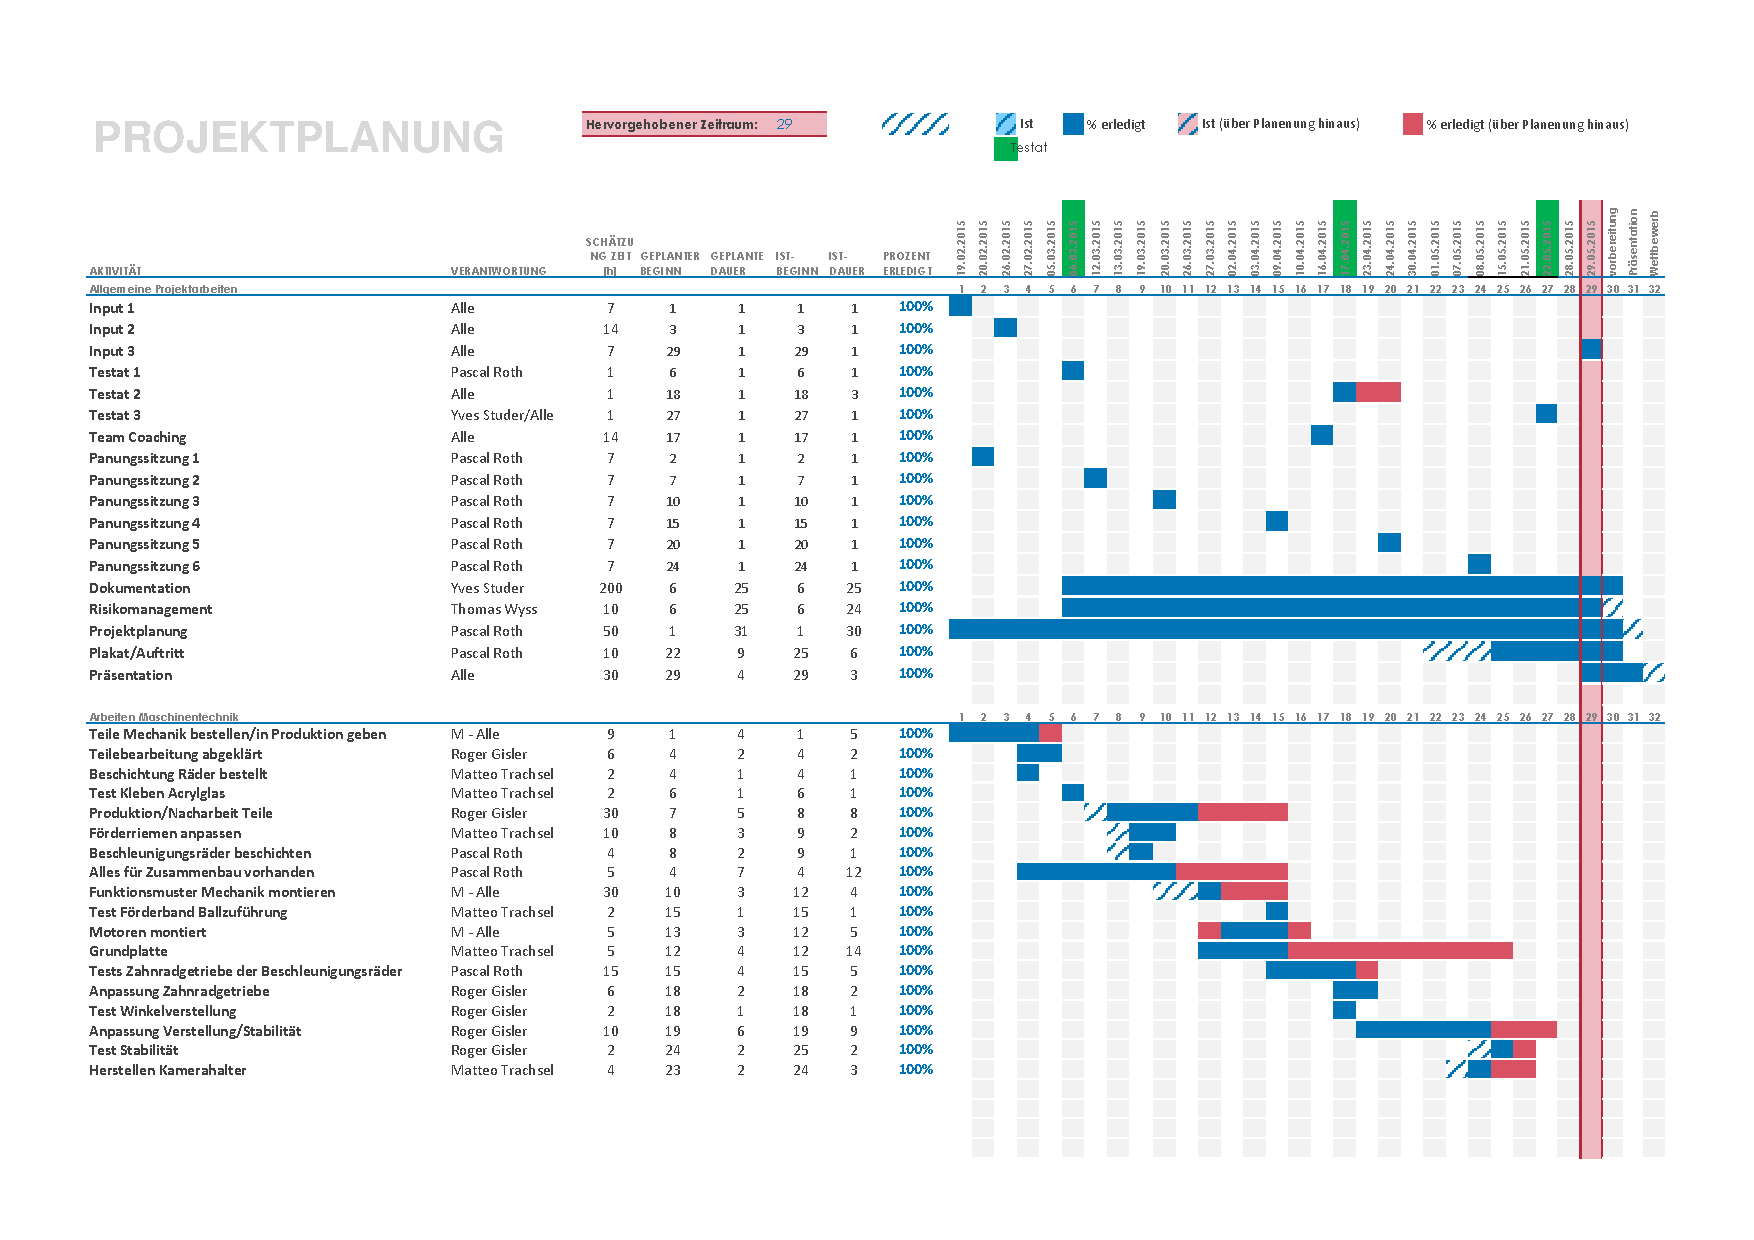
\includegraphics[page=1,scale=0.87,clip,trim=15mm 15mm 13mm 18mm] {Enddokumentation/Bilder/Projektplanung.pdf}
    \newpage        
    \includegraphics[page=2,scale=0.87,clip,trim=15mm 0mm 13mm 10mm] {Enddokumentation/Bilder/Projektplanung.pdf}
\end{landscape}
